%---------------------------0-----------------------------------

\begin{frame}[c]{Geodengue}
\begin{center}
    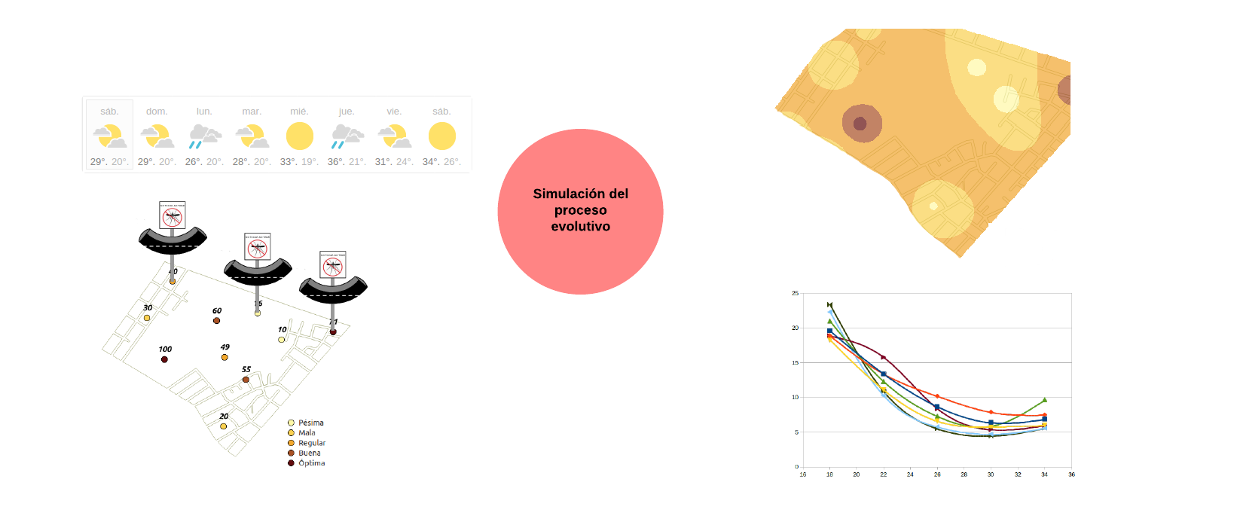
\includegraphics[width=\textwidth]{./graphics/propuesta.png}
\end{center}
\end{frame}

%---------------------------1-----------------------------------

\begin{frame}[c]{Geodengue. Vigilancia Entomológica.}
\begin{center}
    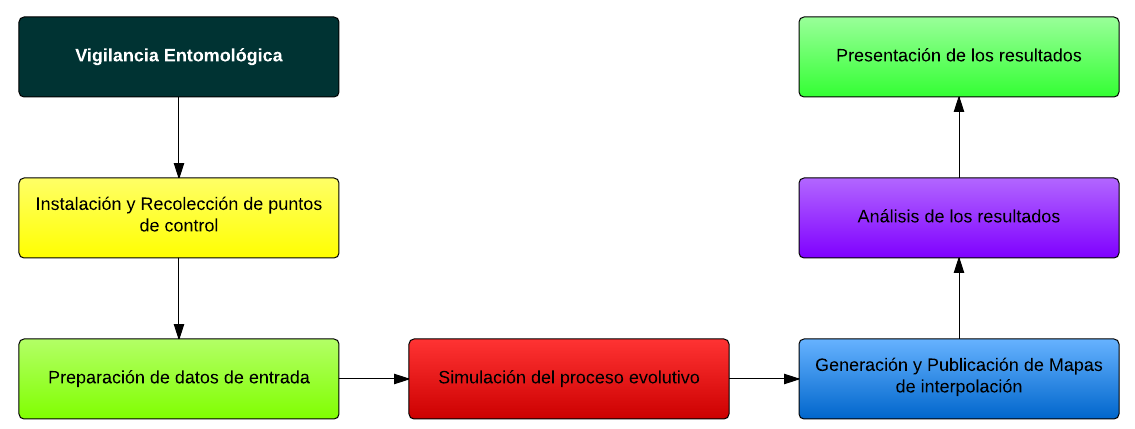
\includegraphics[width=\textwidth]{./graphics/propuesta-vigilancia-entomologica.png}
\end{center}
\end{frame}

\begin{frame}[t]{Vigilancia Entomológica. Larvitrampas}
  \begin{center}
    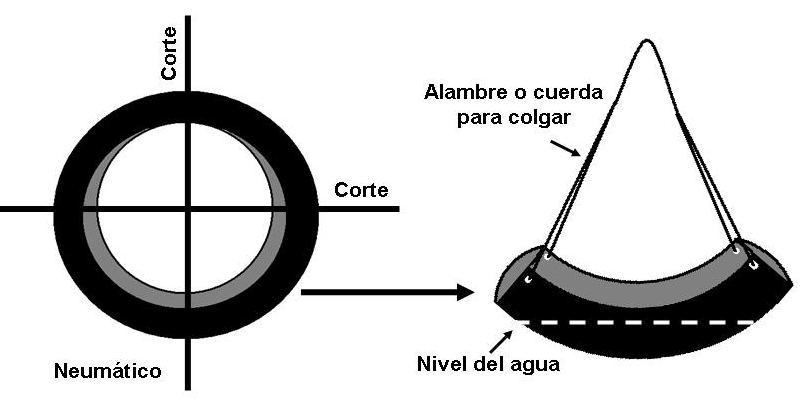
\includegraphics[height=3cm]{../book/anexos/graphics/construccion-larvitrampa.png}
    \begin{itemize}
      \item Se basan en la detección del vector en su etapa larval.
      \item Brinda información sobre los patrones de actividad espacial y estacional de ovipostura.
      \item Permiten reconocer las condiciones climáticas favorables para la eclosión y desarrollo larvario.
    \end{itemize}
  \end{center}
\end{frame}

%----------------------------2----------------------------------

\begin{frame}[c]{Geodengue. Instalación y recolección de puntos de control}
\begin{center}
    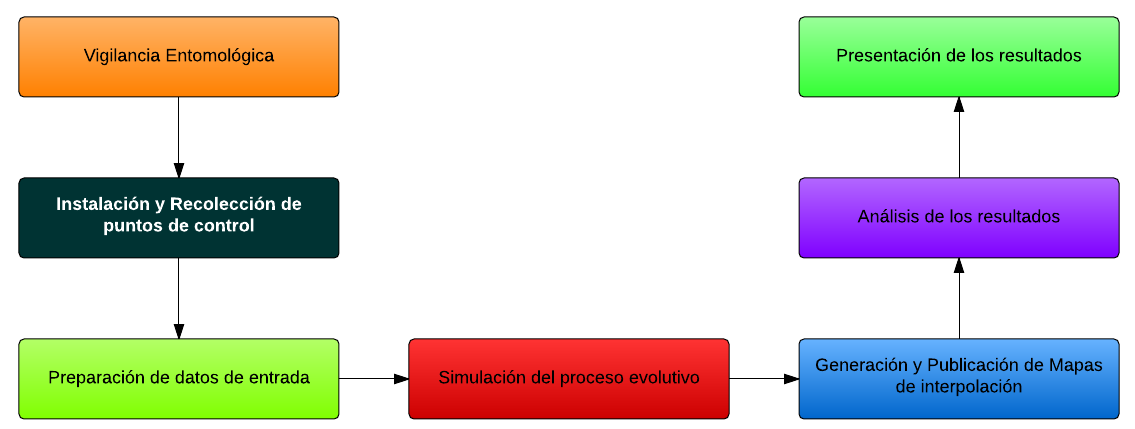
\includegraphics[width=\textwidth]{./graphics/propuesta-puntos-control.png}
\end{center}
\end{frame}

\begin{frame}[c]{Instalación y recolección de puntos de control}
  \begin{center}
    \begin{itemize}
      \item Selección del área de estudio.
      \item Distribución geográfica de los puntos de control.
      \item Revisión de los puntos de control.
      \item Conteo de larvas mediante PDI.
    \end{itemize}
  \end{center}
\end{frame}
%-----------------------------3---------------------------------

\begin{frame}[c]{Geodengue. Preparación de datos de entrada}
\begin{center}
    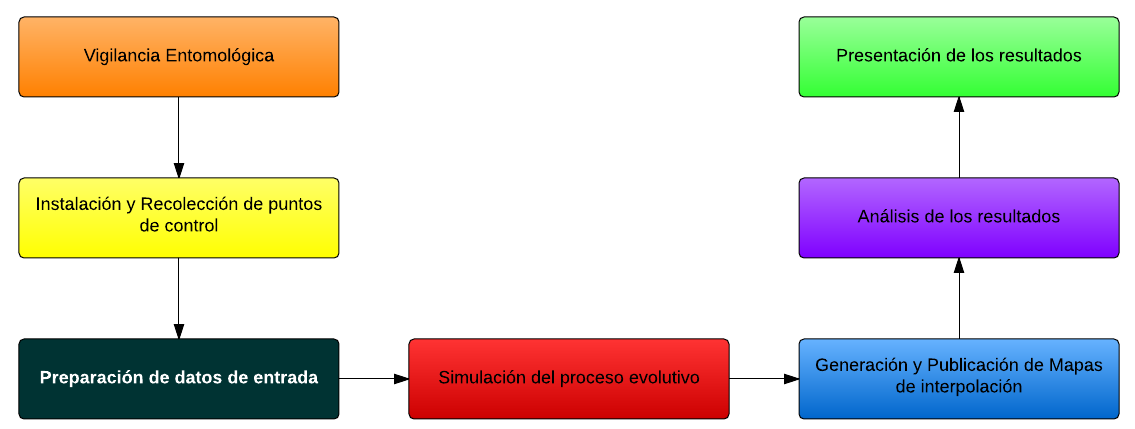
\includegraphics[width=\textwidth]{./graphics/propuesta-datos-entrada.png}
\end{center}
\end{frame}

\begin{frame}[c]{Preparación de datos de entrada}
\begin{columns}[c]
        \begin{column}[c]{4cm}
            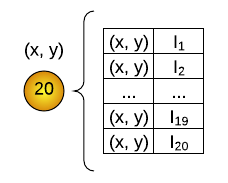
\includegraphics[width=4cm]{./graphics/punto-to-array.png}
        \end{column}
        \begin{column}[c]{6cm}
    \begin{itemize}
      \item Generación de la población inicial a partir de los puntos de control.
      \item Selecciónar periodo de simulación.
      \item Obtener datos climáticos.
    \end{itemize}
    \end{column}
\end{columns}
\end{frame}

%---------------------------4-----------------------------------
\begin{frame}[c]{Geodengue. Simulación del proceso evolutivo}
\begin{center}
    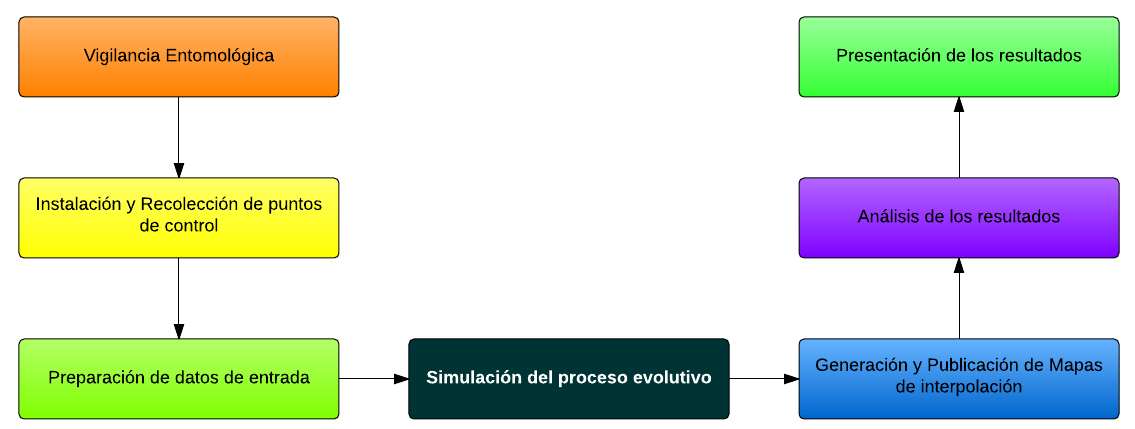
\includegraphics[width=\textwidth]{./graphics/propuesta-simulacion.png}
\end{center}
\end{frame}

\begin{frame}[c]{Simulación del proceso evolutivo}
  \begin{itemize}
    \item Tasas de desarrollo para la eclosión de huevos, larvas, pupas y el ciclo gonotrófico de las hembras adultas.
    \item Mortalidad de huevos, larvas, pupas y mosquitos adultos.
    \item Dispersión de adultos.
    \item Ovipostura de hembras adultas nulíperas y paridas.
    \item Distribución de sexo.
  \end{itemize}
\end{frame}

\begin{frame}[c]{Simulación del proceso evolutivo. Tasas de desarrollo}
  \begin{itemize}
    \item Las tasas dependen no sólo de valores de la población, sino también de la temperatura lo que introduce una dependencia del tiempo.
    \item Se consideran 4 tasas de desarrollos : la eclosión de huevos, emergencia a pupas, emergencia a adultos y el ciclo gonotrófico.
    \item El cálculo de las tasas de desarrollo se realiza mediante el modelo no lineal de Sharpe y DeMichele.
    \item El modelo de Sharpe y DeMichele debe ajustarse con los datos biológicos disponibles.
    \item El modelo de Sharpe y DeMichele puede utilizarse para calcular tasas de desarrollo a cualquier temperatura.
  \end{itemize}
\end{frame}

\begin{frame}[c]{Simulación del proceso evolutivo. Tasas de desarrollo}
\begin{center}
    \begin{equation} \label{eq:schoolfield}
       R(k)  = R(298K) *\cfrac{ \cfrac{k}{298K} *
        exp \Bigg[
                \cfrac{\Delta H_{A}}{R} \bigg(\cfrac{1}{298K} - \cfrac{1}{k}\bigg)
            \Bigg]}
        {1 + exp\Bigg[\cfrac{\Delta H_{H}}{R} \bigg(\cfrac{1}{T_{1/2}}- \cfrac{1}{k}\bigg)\Bigg] }
    \end{equation}
\end{center}
Donde :
 \begin{itemize}
    \item $R(k)$ : Tasa de desarrollo media ($dias^{-1}$).
    \item $\Delta H_{A}$ y $\Delta H_{H}$ : son entalpías termodinámicas características del organismo.
    \item $T_{1/2}$ es la temperatura cuando la mitad de la enzima se desactiva.
    \item $R$ : es la constante universal de los gases.
    \item $k$ : Temperatura en Kelvin.
    \end{itemize}
\end{frame}

\begin{frame}[c]{Simulación del proceso evolutivo. Mortalidad}
  \begin{itemize}
    \item Huevos, es definida como una constante independiente de la temperatura igual a $0.01$\ $1/\text{días}$.
    \item Larvas, expresada como una función, compuesta por la mortalidad bajo óptimas condiciones y la mortalidad denso dependiente.
    \item Pupas, expresada como una función compuesta por la mortalidad bajo óptimas condiciones.
    \item Adultos, es definida como una constante independiente de la temperatura igual a $0.09$\ $1/\text{días}$.
  \end{itemize}
\end{frame}

\begin{frame}[c]{Simulación del proceso evolutivo. Mortalidad}
  Mortalidad de los huevos :
  \begin{center}
      \begin{equation}
          M_{H(x,y)} = me * H(x,y)
      \end{equation}
  \end{center}
  Donde :
    \begin{itemize}
      \item $me$ : Tasa de mortalidad diaria igual a $0,01$ \ $1/\text{días}$.
      \item $H(x, y)$ : Cantidad de huevos observados en $(x,y)$.
      \item $M_{H(x,y)}$ : Cantidad de huevos a eliminar.
    \end{itemize}
\end{frame}

\begin{frame}[c]{Simulación del proceso evolutivo. Mortalidad.}
 Mortalidad bajo optimas condiciones :
\begin{center}
  \begin{equation}
  \label{eq:mortalidad-natural-larvas}
      mo(k) = 0.01 + 0.9725 * exp\bigg( \frac{-(k - 278)}{2.7035}\bigg)
  \end{equation}
\end{center}
Donde :
  \begin{itemize}
    \item $k$ : Temperatura en Kelvin.
  \end{itemize}
\end{frame}

\begin{frame}[c]{Simulación del proceso evolutivo. Mortalidad.}
Mortalidad de las larvas :
  \begin{center}
      \begin{equation}
      M_{L(x,y)}(k) = mo(k) * L(x,y) + \bigg(\frac{\alpha _{0}}{BS(x,y)}\bigg) * L(x,y) *(L(x,y) - 1)
    \end{equation}
  \end{center}
  Donde:
 \begin{itemize}
      \item $k$ : Temperatura en Kelvin.
      \item $L(x, y)$ : Cantidad de larvas observadas en $(x,y)$.
      \item $\alpha _{0}$ : Capacidad de carga de un solo lugar de reproducción.
      \item $BS(x,y)$ : Es el número de sitios de reproducción en $(x,y)$ .
      \item $M_{L(x,y)}$ : Cantidad de larvas a eliminar.
    \end{itemize}
\end{frame}

\begin{frame}[c]{Simulación del proceso evolutivo. Mortalidad.}
Mortalidad de las pupas :
\begin{center}
  \begin{equation}
      M_{P(x,y)}(k) = P(x,y) * (mo(k) + (1 - ef) * R(k))
  \end{equation}
\end{center}
Donde :
  \begin{itemize}
    \item $k$ : Temperatura en Kelvin.
    \item $ef$ : el factor de supervivencia es de $0,83$.
    \item $P(x, y)$ : Cantidad de pupas observadas en $(x,y)$.
    \item $M_{P(x,y)}$ : Cantidad de pupas a eliminar.
  \end{itemize}
\end{frame}

\begin{frame}[c]{Simulación del proceso evolutivo. Mortalidad.}
  Mortalidad de adultos :
  \begin{center}
    \begin{equation}
        M_{A(x,y)} = ma * A(x,y)
    \end{equation}
  \end{center}
  Donde:
    \begin{itemize}
      \item $ma$ : Tasa de mortalidad diaria igual a $0,09$ \ $1/\text{días}$.
      \item $A(x, y)$ : Cantidad de adultos observados en $(x,y)$.
      \item $M_{A(x,y)}$ : Cantidad de adultos a eliminar.
    \end{itemize}
\end{frame}


\begin{frame}[t]{Simulación del proceso evolutivo. Ciclo gonotrófico y Ovipostura.}
  \begin{itemize}
    \item La cantidad de huevos en cada oviposición varía entre 30 y 100 unidades.
    \item La duración del ciclo gonotrófico para hembras nulíperas y paridas.
    \item Las hembras nulíperas poseen un proceso de digestión más lento.
    \item Las tasas de desarrollo para el ciclo gonotrófico para hembras nulíperas y paridas son distintas.
  \end{itemize}
\end{frame}


\begin{frame}[t]{Simulación del proceso evolutivo. Dispersión.}
  \begin{itemize}
    \item El Aedes aegypti es un mosquito doméstico que generalmente.
    \item El mosquito, no sobrepasa los 100 metros de dispersión durante su vida.
    \item En caso de no contar con condiciones favorables tiene a dispersarse hasta 3 kilómetros.
    \item Vuela en sentido contraria a la dirección al viento.
    \item Velocidad máxima de 2 kilómetros por hora.
    \item La dispersión de un mosquito adulto depende de la zona en la que se encuentra.
  \end{itemize}
\end{frame}


\begin{frame}[c]{Simulación del proceso evolutivo}
\begin{center}
  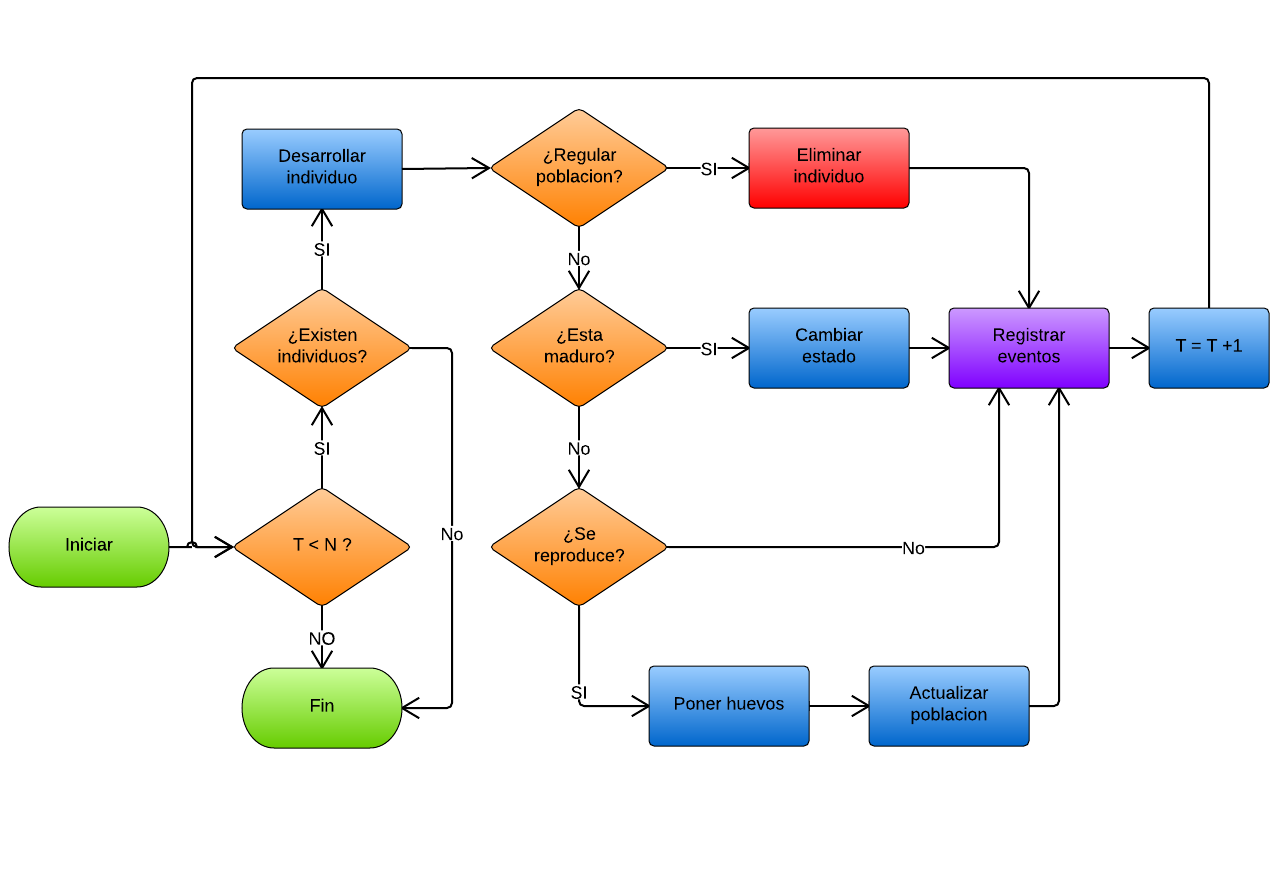
\includegraphics[height=7.5cm]{./graphics/algoritmo-propuesto.png}
\end{center}
\end{frame}

%--------------------------5------------------------------------
\begin{frame}[c]{Geodengue. Generación y publicación de Mapas de interpolación}
\begin{center}
    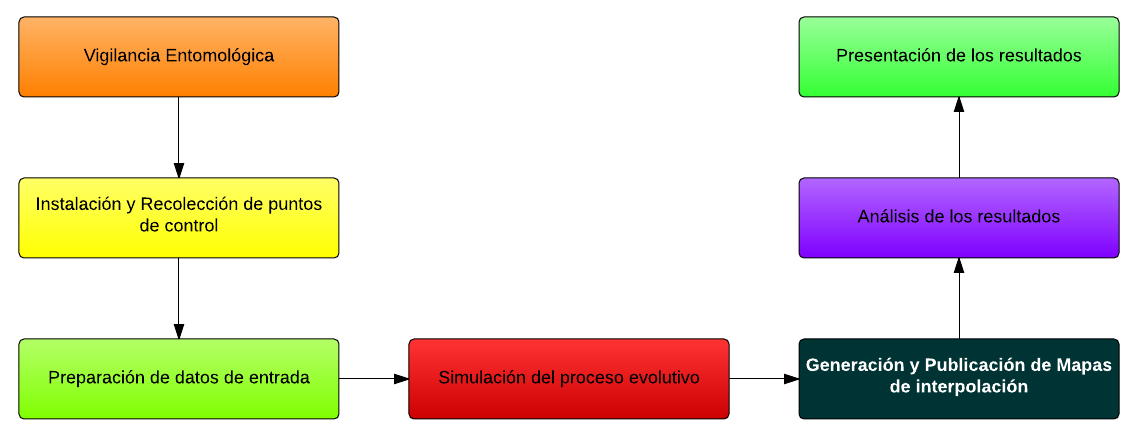
\includegraphics[width=\textwidth]{./graphics/propuesta-mapas.png}
\end{center}
\end{frame}

\begin{frame}[c]{Generación y publicación de Mapas de interpolación}
\begin{center}
    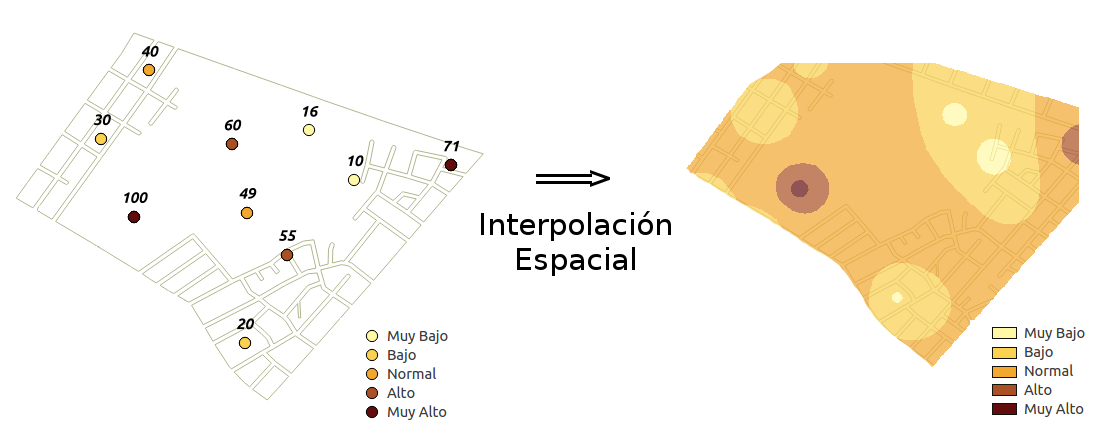
\includegraphics[width=\textwidth]{./graphics/identificacion-focos.png}
    \begin{itemize}
      \item Selección de individuos.
      \item Interpolación espacial de los individuos de la población.
      \item Publicación de capas en el Geoserver.
    \end{itemize}
\end{center}
\end{frame}

%--------------------------6------------------------------------
\begin{frame}[c]{Geodengue. Análisis de los resultados}
\begin{center}
    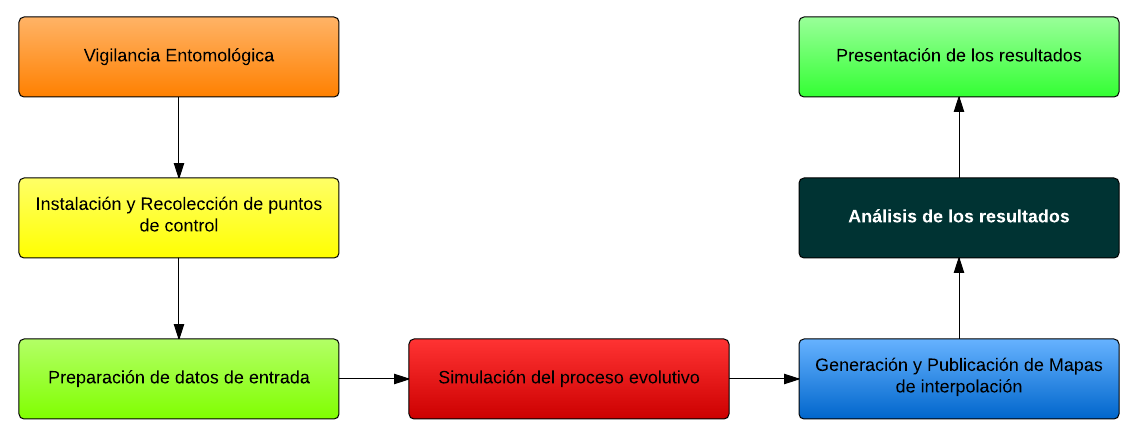
\includegraphics[width=\textwidth]{./graphics/propuesta-analisis.png}
\end{center}
\end{frame}

\begin{frame}[t]{Análisis de los resultados}
\begin{center}
    \begin{itemize}
      \item Tasa promedio de desarrollo.
      \item Tasa promedio de mortalidad diaria.
      \item Cantidad promedio de huevos.
      \item Dispersión media.
      \item Cartografía del vector.
      \item Mapas de interpolación.
    \end{itemize}
\end{center}
\end{frame}

%--------------------------7------------------------------------
\begin{frame}[c]{Geodengue. Presentación de los resultados}
\begin{center}
    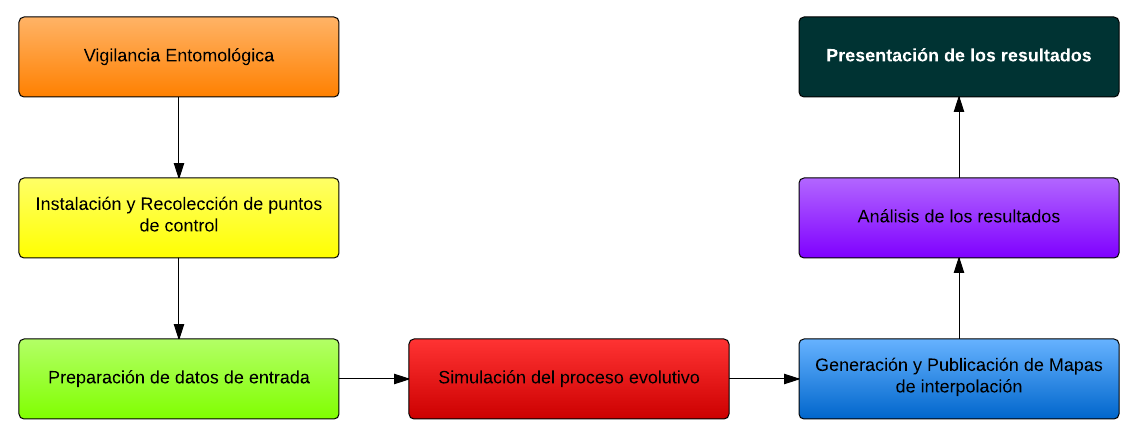
\includegraphics[width=\textwidth]{./graphics/propuesta-resultados.png}
\end{center}
\end{frame}

\begin{frame}[t]{Presentación de los resultados}
  \begin{itemize}
    \item Gráficos explicativos.
    \item Tablas detalladas.
    \item Mapas de interpolación como capas raster.
    \item Objetos puntuales como capas vectoriales.
  \end{itemize}
\end{frame}
